%!TEX TS-program = xelatex
\documentclass[]{friggeri-cv}
\usepackage{afterpage}
\usepackage{hyperref}
\usepackage{color}
\usepackage{xcolor}
\hypersetup{
    pdftitle={Md Abdul Hasib},
    pdfauthor={},
    pdfsubject={},
    pdfkeywords={},
    colorlinks=false,       % no lik border color
   allbordercolors=white    % white border color for all
}
\addbibresource{bibliography.bib}
\RequirePackage{xcolor}
\definecolor{pblue}{HTML}{0395DE}

\begin{document}
\header{Md}{ Abdul Hasib}
      {Full Stack ML Engineer|Team Lead}
      
% Fake text to add separator      
\fcolorbox{white}{gray}{\parbox{\dimexpr\textwidth-2\fboxsep-2\fboxrule}{%
.....
}}

% In the aside, each new line forces a line break
\begin{aside}
  \section{Address}
    South Mugda
    Dhaka, Bangladesh
    ~
  \section{Tel \& Skype}
    +8801917187787
    live:abdulhasibsazzad
    ~
  \section{Mail}
    \href{mailto:abdulhasibsazzad@gmail.com}{\textbf{abdulhasibsazzad@}\\gmail.com}
    \href{mailto:abdulhasibsazzad@.hotmail.com}{\textbf{abdulhasibsazzad@}\\hotmail.com}
    ~
  \section{Web \& Git}
    \href{http://www.abdulhasibsazzad.com}{abdulhasibsazzad.com}
    \href{https://bitbucket.org/neoben}{bitbucket.org/neoben}
    \href{https://github.com/sazzadBuet08}{github.com/sazzadBuet08}
    ~
  \section{Programming}
    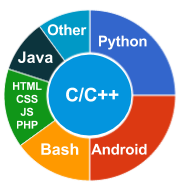
\includegraphics[scale=0.62]{img/programming.png}
    ~
  %\section{OS Preference}
   % \textbf{Ubuntu}
\includegraphics[scale=0.40]{img/5stars.png}
    %\textbf{MacOS}
\includegraphics[scale=0.40]{img/4stars.png}
    %\textbf{Windows}
\includegraphics[scale=0.40]{img/3stars.png}
    %~
  \section{Personal Skills}
    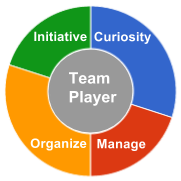
\includegraphics[scale=0.62]{img/personal.png}
    ~
  \section{Languages}
    \textbf{Italian}
\includegraphics[scale=0.40]{img/5stars.png}
    \textbf{English}
\includegraphics[scale=0.40]{img/4stars.png}
    ~
\end{aside}

\section{Experience}
\begin{entrylist}
  \entry
    {10/16 - Now}
    {Senior Software and ML Engineer}
    {Infolytx Inc, Bangladesh}
    {Took ownership of the product as well as the whole team.
    Disseminated knowledge of architectural patterns and coding best practices for both client and server development.
Collaborated with architect and infrastructure teams to maintain technical consistency across multiple products.
Completed CSM and worked as a ScrumMaster and Team Lead on some projects.\\}
    \entry
    {08/15 - 10/16}
    {Software Engnieer}
    {Infolytx Inc, Bangladesh}
    {Worked on different machine learning based solution.
Worked with UMLS dictionaries and HL7 standards.
Analyzing electronic medical records.
Analyzing large clinical data sets in MongoDB.
Natural language processing in the clinical context (Java).
Building web services / APIs (Java).
Building front-end prototypes with Ruby on Rails and React. 
Working on various Java applications - core project work, utilities, etc.
\\}
    \entry
    {08/14 - 08/15}
    {Junior Software Engineer}
    {Nascenia Inc, Bangladesh}
    {Worked as a team player to develop a web application with on Ruby on rails
Developed some projects solely from initial requirement gathering to design, coding, testing,
Did documentation and implementation and client handling.
Worked with the application server, web server, and Jenkins server.
Handled and provided API services. 
Took Technical Session on Git, Clean Code, Active Record Query. \\}
\end{entrylist}

\section{Education}
\begin{entrylist}
  \entry
    {2009 - 2014}
    {B.Sc. in Computer Engineering}
    {Bangladesh University of Engineering and Technology}
    {Curriculum Networking and Multimedia.\\
    Main subjects: Network Applications, Systems Architecture and Security, Mobile Applications, Multemedia Information            Processing.\\
    \emph{Title of the Thesis: "A Handoff Algorithm based on Link Quality Prediction for Mass Transit Wireless Mesh Networks"      .}\\
    \emph{Relators: Prof. Enzo Mingozzi, Ing. Carlo Vallati, Prof. Luciano Lenzini.}\\}
\end{entrylist}

\section{Certifications}
\begin{entrylist}
  \entry
    {02/2013}
    {Intro to Computer Science}
    {Udacity. E-learning}
    {\emph{Building a Python Search Engine}}
\end{entrylist}

%\begin{flushleft}
%\emph{January 14th, 2014}
%\end{flushleft}
%\begin{flushright}
%\emph{Carmine Benedetto}
%\end{flushright}
%\newpage

%\begin{aside}
  %\section{Languages}
    %\textbf{Italian}
\includegraphics[scale=0.40]{img/5stars.png}
    %\textbf{English}
\includegraphics[scale=0.40]{img/4stars.png}
%\end{aside}

%%% This piece of code has been commented by Karol Kozioł due to biblatex errors. 
% 
%\printbibsection{article}{article in peer-reviewed journal}
%\begin{refsection}
%  \nocite{*}
%  \printbibliography[sorting=chronological, type=inproceedings, title={international peer-reviewed conferences/proceedings}, notkeyword={france}, heading=subbibliography]
%\end{refsection}
%\begin{refsection}
%  \nocite{*}
%  \printbibliography[sorting=chronological, type=inproceedings, title={local peer-reviewed conferences/proceedings}, keyword={france}, heading=subbibliography]
%\end{refsection}
%\printbibsection{misc}{other publications}
%\printbibsection{report}{research reports}

\end{document}
